%%% template.tex
%%%
%%% This LaTeX source document can be used as the basis for your technical
%%% paper or abstract. Regardless of the length of your document, the commands
%%% are all the same.
%%% 
%%% The "\documentclass" command is the first command in your file. If you want to 
%%% prepare a version of your article with line numbers - a "review" version - 
%%% include the "review" parameter:
%%%    \documentclass[review]{acmsiggraph}
%%%


%\documentclass{article}
\documentclass{acmsiggraph}
%\documentclass[compsoc]{IEEEtran}{acmsiggraph}

% this package is to add marging left ... for the Titles 
%and it should match this Format \titlespacing*{<command>}{<left>}{<before-sep>}{<after-sep>} 
% see link: http://tex.stackexchange.com/questions/108684/spacing-before-and-after-section-titles
\usepackage{blindtext}

%this package is to manage the Sectioning and its numerals( Roman, alpha arabic )
% see link  http://tex.stackexchange.com/questions/3177/how-to-change-the-numbering-of-part-chapter-section-to alphabetical-r
\usepackage{titlesec}

% to fix the widths of columns in Tabulor
\usepackage{array}
\newcolumntype{L}[1]{>{\raggedright\let\newline\\\arraybackslash\hspace{0pt}}m{#1}}
\newcolumntype{C}[1]{>{\centering\let\newline\\\arraybackslash\hspace{0pt}}m{#1}}
\newcolumntype{R}[1]{>{\raggedleft\let\newline\\\arraybackslash\hspace{0pt}}m{#1}}

% to write umlaute
\usepackage[utf8]{inputenc}
%http://tex.stackexchange.com/questions/161431/how-to-solve-longtable-is-not-in-1-column-mode-error
%\usepackage{supertabular,booktabs}
\usepackage{xtab,booktabs}  
% prevent tables from being broken too early
%http://tex.stackexchange.com/questions/15876/prevent-xtab-breaking-table-too-soon
\xentrystretch{-0.1}
% increase spacing between table's rows
\renewcommand{\arraystretch}{1.2}


%%% Title of your article or abstract.

\title{Evaluating a Representational State Transfer (REST) Architecture: What is the Impact of REST in My Architecture?}

\author{Jawhar Ben Hadj M'barek\thanks{e-mail:spencer@cs.washington.edu}\\Chair, ACM SIGGRAPH Publications Committee}
\pdfauthor{Stephen N. Spencer}

%%% Used by the ``review'' variation; the online ID will be printed on 
%%% every page of the content.

\TOGonlineid{45678}

% User-generated keywords.

\keywords{radiosity, global illumination, constant time}

% With the "\setcopyright" command the appropriate rights management text will be added
% to your document.

%\setcopyright{none}
%\setcopyright{acmcopyright}
%\setcopyright{acmlicensed}
\setcopyright{rightsretained}
%\setcopyright{usgov}
%\setcopyright{usgovmixed}
%\setcopyright{cagov}
%\setcopyright{cagovmixed}
%\setcopyright{rightsretained}

% The year of publication in the "\copyrightyear" command.

\copyrightyear{2016}

%%% Conference information, from the completed rights management form.
%%% The "\conferenceinfo" command has two parameters: 
%%%    - conference name
%%%    - conference date and location
%%% The "\isbn" field includes the year and month after the article ISBN.

\conferenceinfo{SIGGRAPH 2016 Posters}{July 24-28, 2016, Anaheim, CA} 
\isbn{978-1-4503-ABCD-E/16/07} 
\doi{http://doi.acm.org/10.1145/9999997.9999999}

\begin{document}
% Sectioning
\renewcommand{\thesection}{\Roman{section}.} 
\renewcommand{\thesubsection}{\Alph{subsection}.}
\renewcommand{\thesubsubsection}{\arabic{subsubsection})}

\titlespacing*{\section}
{0pt}{0\baselineskip}{0\baselineskip}
%{0pt}{5.5ex plus 1ex minus .2ex}{4.3ex plus .2ex}
\titlespacing*{\subsection}
{5pt}{0\baselineskip}{0\baselineskip}
\titlespacing*{\subsubsection}
{10pt}{0\baselineskip}{0\baselineskip}

\titleformat*{\section}{\large\bfseries}
\titleformat*{\subsection}{\large\bfseries}
\titleformat*{\subsubsection}{\fontencoding{OT1}\fontfamily{cmr}\fontseries{m}%
  \fontshape{n}\fontsize{9pt}{9}\selectfont\slshape}





%%% This is the ``teaser'' command, which puts an figure, centered, below 
%%% the title and author information, and above the body of the content.

 \teaser{
   \includegraphics[height=1.5in]{images/sampleteaser}
   \caption{Spring Training 2009, Peoria, AZ.}
 }

\maketitle
\begin{abstract}

In this sample paper, we describe the formatting requirements for
content accepted to SIGGRAPH-sponsored events. The same format can be
used for content ranging from a one- or two-page Poster or Talk abstract, to a
full-length Technical Paper. 

[New for 2016] Authors are now responsible for adding the appropriate rights management
text to their final content, by adding information found on one's completed 
rights management form to the source document.

[New for 2016] Authors are now required to use ACM's current Computing Classification
System for the inclusion of appropriate subject concepts.

Please view the accompanying README file for a complete description of the formatting
specifications.

\end{abstract}

%
% The code below should be generated by the tool at
% http://dl.acm.org/ccs.cfm
% Please copy and paste the code instead of the example below. 
%
\begin{CCSXML}
<ccs2012>
<concept>
<concept_id>10010147.10010371.10010382</concept_id>
<concept_desc>Computing methodologies~Image manipulation</concept_desc>
<concept_significance>500</concept_significance>
</concept>
<concept>
<concept_id>10010147.10010371.10010382.10010236</concept_id>
<concept_desc>Computing methodologies~Computational photography</concept_desc>
<concept_significance>300</concept_significance>
</concept>
</ccs2012>
\end{CCSXML}

\ccsdesc[500]{Computing methodologies~Image manipulation}
\ccsdesc[300]{Computing methodologies~Computational photography}

%
% End generated code
%

% The next three commands are required, and insert the user-generated keywords, 
% The CCS concepts list, and the rights management text.
% Please make sure there is a blank line between each of these three commands.

\keywordlist

\conceptlist

\printcopyright

\section{First Section Headinggggg}

Ut sagittis arcu ut turpis sodales, nec venenatis magna efficitur. Fusce non rhoncus risus, ac tincidunt arcu. Nulla lacus odio, accumsan tempor dolor sit amet, tincidunt porttitor justo. Quisque vulputate ex ac purus ultrices tristique. Pellentesque habitant morbi tristique senectus et netus et malesuada fames ac turpis egestas. Curabitur sed ullamcorper metus. Phasellus eu purus eget leo vulputate auctor vel scelerisque velit.

%\begin{table}[ht]
 % \centering
 % \caption{A simple table.}
 % \begin{tabular}{|r|l|}
 %   \hline
 %   7C0 & hexadecimal \\
 %   3700 & octal \\ \cline{2-2}
 %   11111000000 & binary \\
 %   \hline \hline
 %   1984 & decimal \\
 %   \hline
 % \end{tabular}
%\end{table}


\begin{table}[ht]
  \centering
  \caption{A second simple table.}
  \begin{tabular}{|C{2cm}|L{5,5cm}|}   
    \hline
    Quality Attribute & Szenario \\
    \hline
    Interoperabilität (Interoperability) & I1 - Ein  Service Verbraucher 'A' ruft eine Ressource 'R1' auf und
erhält die Darstellung (Presentation) des aktuellen  Zustandes von 'R1' in Response-Nachricht.
I2 - Ein Service Verbraucher 'A' ruft eine Ressource 'R1' in einer Spezifisches Format (Medientyp) auf und empfängt die Presentation des aktuellen Zustands von 'R1' als Antwort Nach dem gewünschten Format.
I3 - Ein Service Verbraucher 'A' fordert eine Ressource 'R1' und Kann alle Informationen in der Antwort Nachricht nachvollziehen.
 \\ 
    \hline
    3700 & octal \\ 
    \hline
    11111000000 & binary \\ %\cline{1-2}
    1984 & decimal \\ 
    \hline
  \end{tabular}
\end{table}
  
Etiam sed mattis justo. Mauris lorem sapien, pellentesque vel viverra varius, porta ut nisi. Cras vel interdum dui, vitae fermentum elit. Nulla eu libero finibus, bibendum elit nec, ullamcorper velit. Donec ultrices, purus id ullamcorper euismod, ipsum erat sodales augue, ut sagittis sapien magna nec ex. Nulla massa arcu, suscipit non molestie ut, tristique id tellus. Maecenas nec malesuada mauris, vitae mattis sem. Quisque at risus quis arcu eleifend lacinia non sed neque.

\section{Second Section Heading}

Ut sagittis arcu ut turpis sodales, nec venenatis magna efficitur. Fusce non rhoncus risus, ac tincidunt arcu. Nulla lacus odio, accumsan tempor dolor sit amet, tincidunt porttitor justo. Quisque vulputate ex ac purus ultrices tristique. Pellentesque habitant morbi tristique senectus et netus et malesuada fames ac turpis egestas. Curabitur sed ullamcorper metus. Phasellus eu purus eget leo vulputate auctor vel scelerisque velit.

\subsection{This is a subsection}

\subsubsection{This is a subsubsection 1}
Nunc vitae lorem nec diam ultrices fringilla. Aliquam volutpat metus ut magna bibendum, sed ultricies nunc placerat. Nulla volutpat rutrum vehicula. Cum sociis natoque penatibus et magnis dis parturient montes, nascetur ridiculus mus. Aliquam vel ligula elit. Nulla fermentum purus eu venenatis mollis. Nulla placerat dui accumsan urna pharetra maximus. Sed nec orci arcu. Suspendisse faucibus blandit libero ut feugiat. Nulla vitae imperdiet nulla. Cum sociis natoque penatibus et magnis dis parturient montes, nascetur ridiculus mus.

Etiam sed mattis justo. Mauris lorem sapien, pellentesque vel viverra varius, porta ut nisi. Cras vel interdum dui, vitae fermentum elit. Nulla eu libero finibus, bibendum elit nec, ullamcorper velit. Donec ultrices, purus id ullamcorper euismod, ipsum erat sodales augue, ut sagittis sapien magna nec ex. Nulla massa arcu, suscipit non molestie ut, tristique id tellus. Maecenas nec malesuada mauris, vitae mattis sem. Quisque at risus quis arcu eleifend lacinia non sed neque.

\subsubsection{This is a subsubsection 2}
Nunc vitae lorem nec diam ultrices fringilla. Aliquam volutpat metus ut magna bibendum, sed ultricies nunc placerat. Nulla volutpat rutrum vehicula. Cum sociis natoque penatibus et magnis dis parturient montes, nascetur ridiculus mus. Aliquam vel ligula elit. Nulla fermentum purus eu venenatis mollis. Nulla placerat dui accumsan urna pharetra maximus. Sed nec orci arcu. Suspendisse faucibus blandit libero ut feugiat. Nulla vitae imperdiet nulla. Cum sociis natoque penatibus et magnis dis parturient montes, nascetur ridiculus mus.
\subsection{This is another subsection}

Praesent lacinia, risus eget lacinia elementum, lorem elit ullamcorper arcu, quis condimentum ipsum dui at felis. Mauris maximus at lectus condimentum efficitur. Maecenas luctus, magna nec porttitor semper, justo libero semper nisi, nec commodo nunc turpis a velit. Morbi ac elementum urna, in elementum massa. Mauris ipsum turpis, fringilla in pellentesque a, mattis non erat. Cras vitae sodales lacus. Mauris sit amet laoreet ipsum. Maecenas quis consectetur dui. Nunc vulputate, dui eu blandit volutpat, augue dui molestie risus, et viverra lorem ligula quis eros.

\begin{figure}[ht]
  \centering
  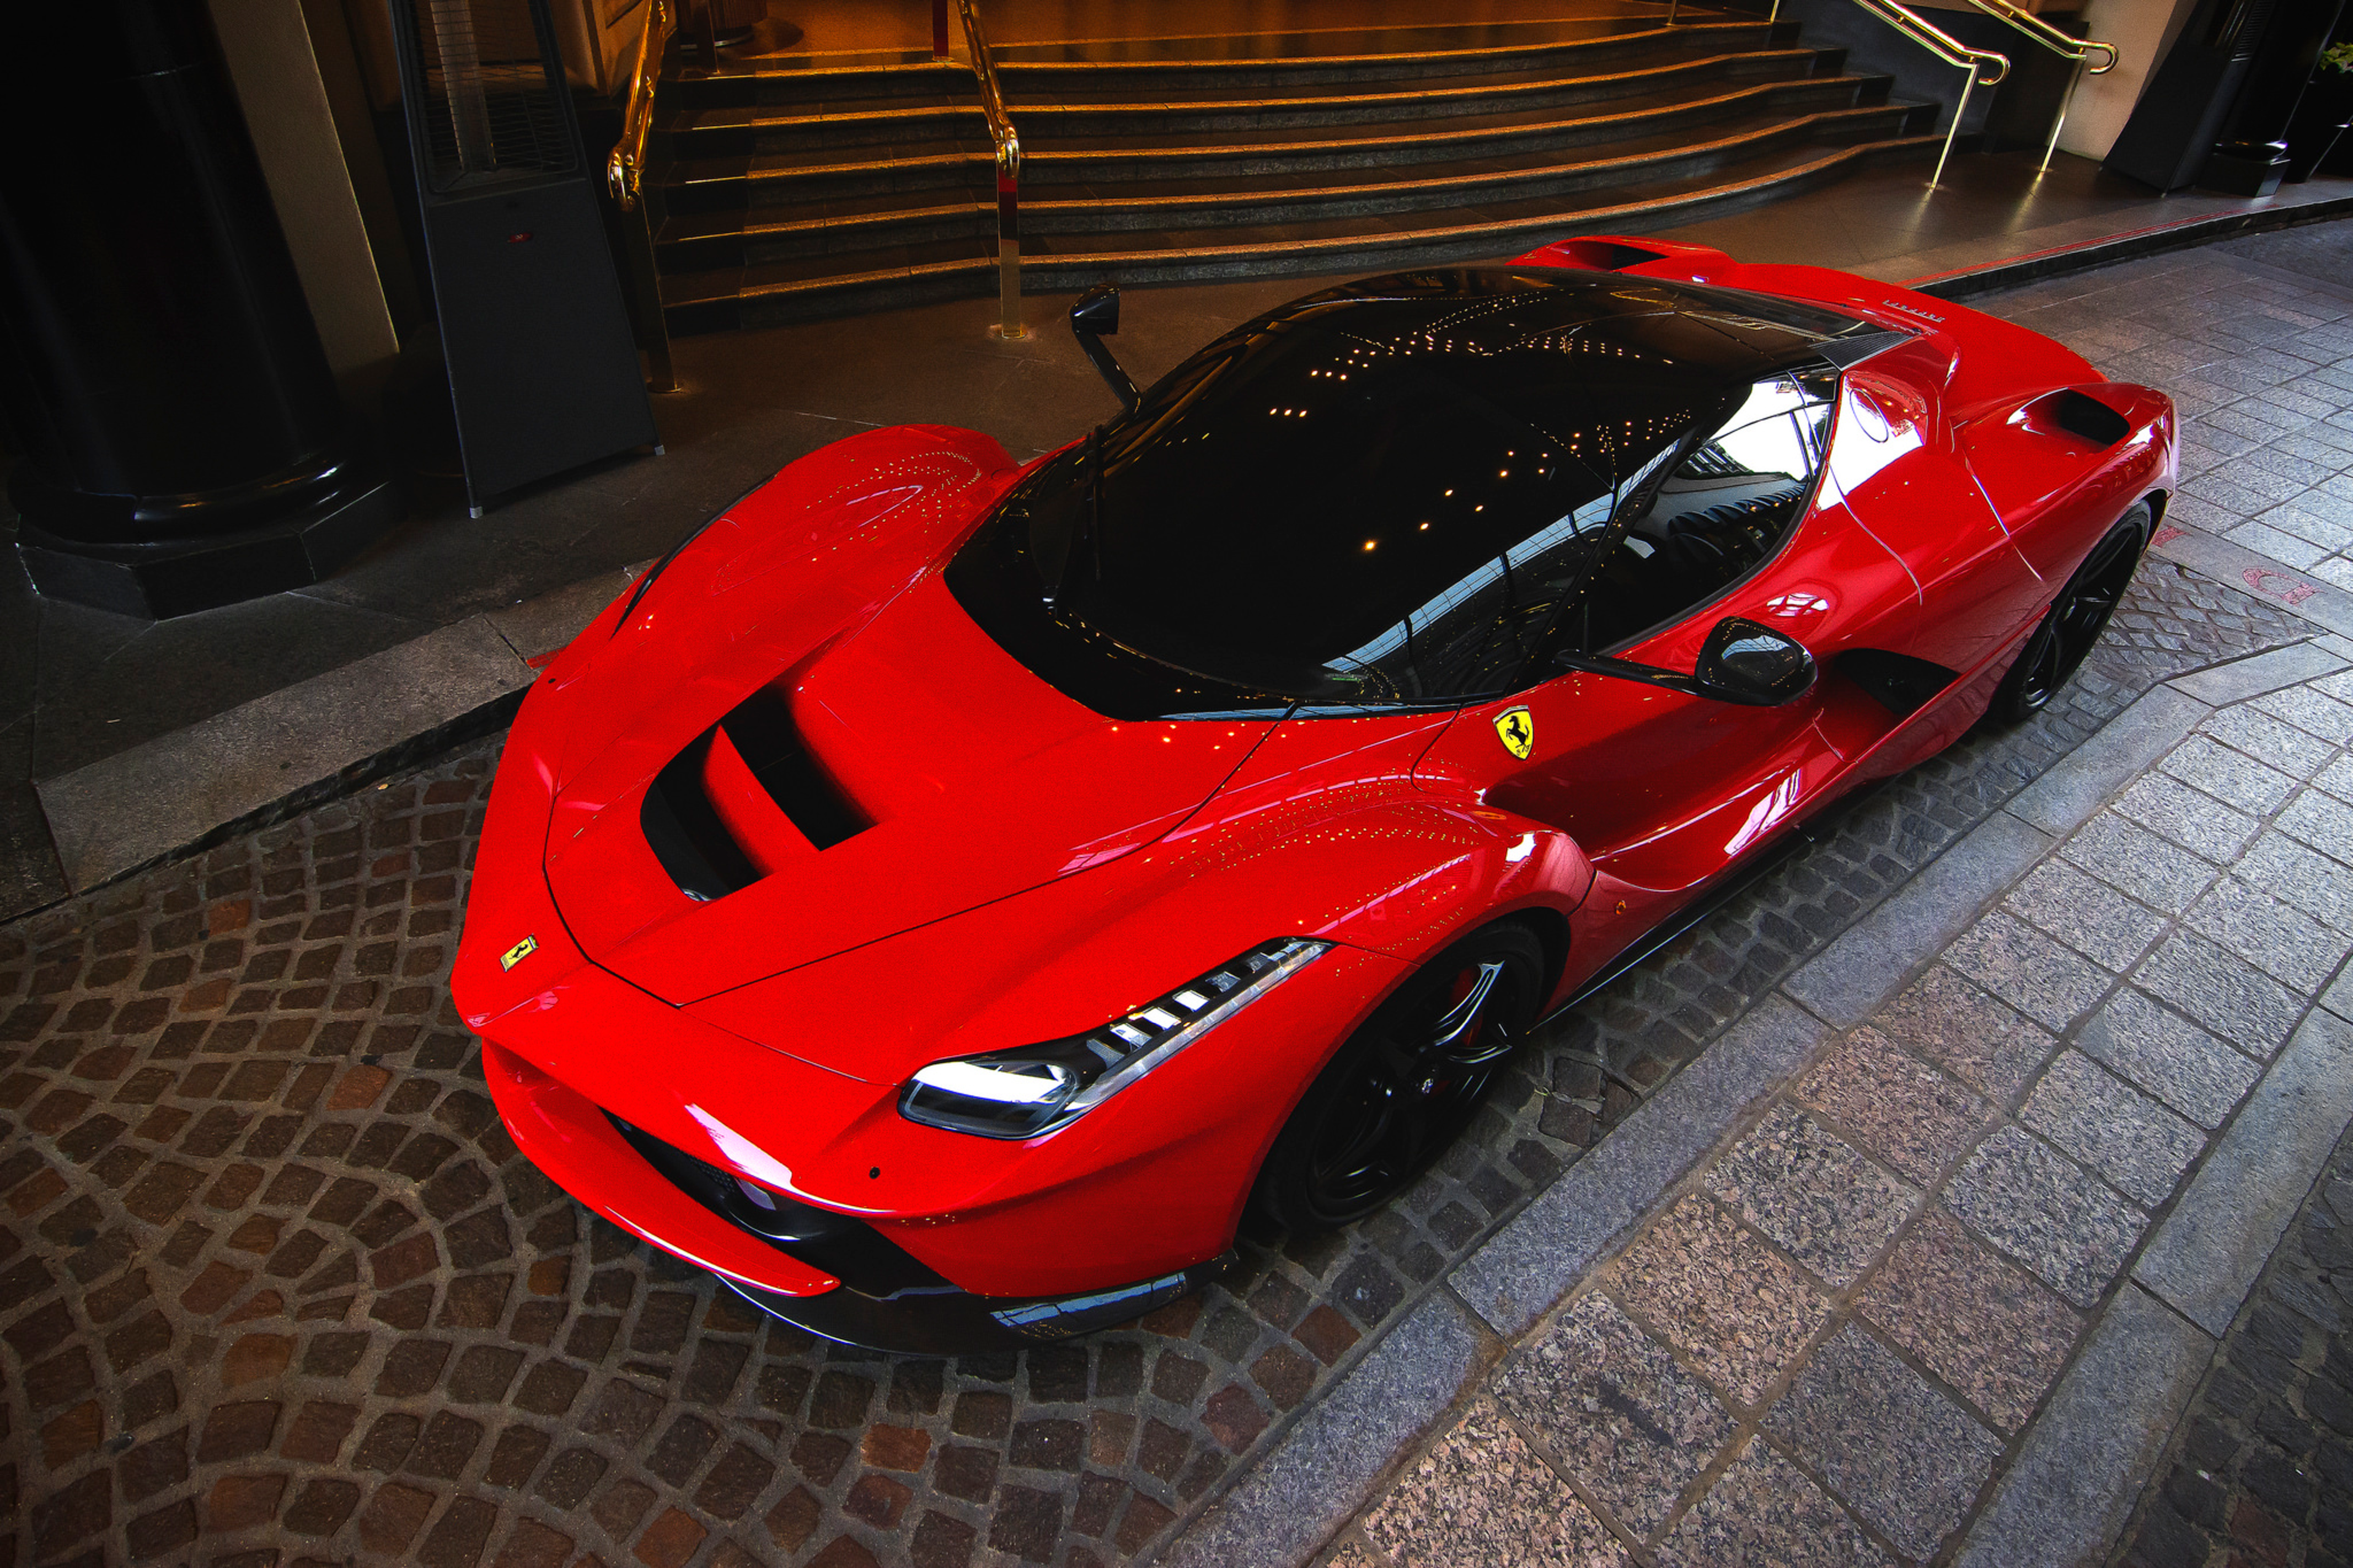
\includegraphics[width=3.0in]{images/ferrari_laferrari}
  \caption{Ferrari LaFerrari. Image courtesy Flickr user ``gfreeman23.''}
  \label{fig:ferrari}
\end{figure}

\section{Third Section Heading}

Ut sagittis arcu ut turpis sodales, nec venenatis magna efficitur. Fusce non rhoncus risus, ac tincidunt arcu. Nulla lacus odio, accumsan tempor dolor sit amet, tincidunt porttitor justo. Quisque vulputate ex ac purus ultrices tristique. Pellentesque habitant morbi tristique senectus et netus et malesuada fames ac turpis egestas. Curabitur sed ullamcorper metus. Phasellus eu purus eget leo vulputate auctor vel scelerisque velit.

Nunc vitae lorem nec diam ultrices fringilla. Aliquam volutpat metus ut magna bibendum, sed ultricies nunc placerat. Nulla volutpat rutrum vehicula. Cum sociis natoque penatibus et magnis dis parturient montes, nascetur ridiculus mus. Aliquam vel ligula elit. Nulla fermentum purus eu venenatis mollis. Nulla placerat dui accumsan urna pharetra maximus. Sed nec orci arcu. Suspendisse faucibus blandit libero ut feugiat. Nulla vitae imperdiet nulla. Cum sociis natoque penatibus et magnis dis parturient montes, nascetur ridiculus mus.

Etiam sed mattis justo. Mauris lorem sapien, pellentesque vel viverra varius, porta ut nisi. Cras vel interdum dui, vitae fermentum elit. Nulla eu libero finibus, bibendum elit nec, ullamcorper velit. Donec ultrices, purus id ullamcorper euismod, ipsum erat sodales augue, ut sagittis sapien magna nec ex. Nulla massa arcu, suscipit non molestie ut, tristique id tellus. Maecenas nec malesuada mauris, vitae mattis sem. Quisque at risus quis arcu eleifend lacinia non sed neque.
\section{GRUNDLAGEN VON REST FÜR ARCHITEKTUR-EVALUIERUNG (EVALUATION CONCERN EC1):}
Eines der Hauptziele einer Architekturbewertung ist die Überprüfen von Risiken, um Attributanforderungen in Software Architektur zu adressieren.
In den nächsten Abschnitte werden die Grundlagen von REST beschrieben unter Berücksichtigung ihrer Auswirkungen in Qualitätsmerkmalen

\subsection{REST Bedingungen:}
Roy Fielding hat sechs Kriterien beschrieben, die den REST-Stil definieren und Jede Einschränkung davon fördert eine andere Reihe von Qualitätsattributen.
REST = (C-S, S, \$, U, L, CoD)
\subsubsection{Client-Server (C-S):}
REST konzentriert sich stark auf die Entkopplung von Client und Server.
Die wichtigsten Vorteile des Client-Server Konzepts sind die Trennung von Verantwortlichkeiten, unabhängige Evolution und Wartbarkeit.
Bewerter sollen die Grenze zwischen Client und Server nach der Zusammenhalt  (cohesion) der unabhängigen Entwicklung von Jeder prüfen.  

\subsubsection{Stateless (S) (der Konversationstatus):}
Das bedeutet, dass kein Konversationsstatus auf dem Server zwischen Requests gehalten wird; der Zustand der Konversation wird auf dem Client gehalten.
Für Evaluators ist der Serverseitiger  Datenfluss  eine wichtige Prüfpunkt.
Die stateless Bedingung ermöglicht die Replikation von Server-Aufrufe und damit fördert die Verfügbarkeit, Skalierbarkeit und Zuverlässigkeit auf Server-Seite. 
Auf der anderen Seite kann die Leistung verringert werden auf Grund der Notwidigkeit, dass  der Konversationsstatus eingebittet in Request and Response versandt muss.

\subsubsection{Cache (\$):}
Ein Cache-Element wirkt als Vermittler zwischen Client und Server. Das Ziel ist es, das Request-Response prozess  zu vermeiden, wenn die Information im Cache vorhanden ist.
Evaluatoren sollen untersuchen, welche Daten zwischengespeichert werden können, und in wie weit kann der Cache die Netzwerkeffizienz verbessern und damit kann die Leistung erhöht werden.
Jedoch kann die Verwendung eines Caches die Zuverlässigkeit (reliability) verringern, insbesondere wenn der Client nicht aktualisierte, alte Daten aus dem Cache verbraucht.

\subsubsection{Uniform Interface (U):}
Uniform Interface ist die zentrale Eigenschaft, die REST von anderen netzwerkbasierten Stilen unterscheidet.
Uniform Interface ist eng mit den Begriffe: Ressourcen, Identifikatoren und Repräsentationen verknüpft.
Eine Ressource ist jedes wichtige Konzept in der Systemdomäne, das wir durch eine uniform Interface erreichbar machen wollen.
Ein Service Consumer adressiert Ressourcen durch einen eindeutigen Identifikator (URI) und eine Repräsentation. Die Darstellung einer Ressource bezieht sich auf ein Hypermedia-Dokument (Text-info, Graphik info,  Animation, Audio Info, video Info…) oder auf einen link zu anderen Ressourcen. (JSON or XML code : HAL - Hypertext Application Language). 
Endlich muss auf die Representation einer Ressource durch eine einfache Interface zugegriffen werden, die eine Identifikation für die Ressource und gemeinsame Methoden( POST, PUT, DELETE, GET ) für den Zugriff definiert. Diese Schnittstelle ist die uniform Interface. Die Uniform interface Bedingung hat einen großen Einfluss auf die Qualitätsmerkmale der Interoperabilität und der Erkennbarkeit. 

\subsubsection{Layered System (L):}
Das Architekturmuster, das leichter die REST-Schicht-Einschränkung identifiziert, ist multi-tier. Es ist von Fielding beschrieben.
Multi-Tier ist ein architektonischer Stil, wobei eine Zwischenstufe als Server für die vorhergehende Stufe und als Client für die nachfolgende Stufe dient.
Diese  Entwurfmuster ist eine Spezialisierung der Client-Server-Stil. 

\subsubsection{Code-on-Demand (CoD) (einzige optionale Bedingung):}	
REST ermöglicht die Erweiterung der Client-Funktionalität durch das Herunterladen und Ausführen von Code in Form von Applets oder Skripten.
Dies vereinfacht die Clients, indem sie die Anzahl der erforderlichen Features reduziert.
Das Zulassen von Features, die nach Deployment heruntergeladen werden können, verbessert die Erweiterbarkeit des Systems (the extensibility).
Allerdings reduziert es auch die Sichtbarkeit (the visibility) und ist somit nur eine optionale Einschränkung innerhalb REST.
Dies ist ein Beispiel für Code-on-Demand : der Browser greift ein initiales HTML-Dokument und unterstützt <script> -Tags innerhalb dieses Dokuments, so dass eine Anwendung on-demand geladen werden kann.
Der Code kann ein Javascript, Java-Applet oder sogar eine Flash-Anwendung sein.

\subsection{Pragmatischer REST:}
Die Bedingungen (C-S, S, \$, U, L, CoD) repräsentieren das, was "Pure REST" genannt wird.
Viele technische Lösungen und Entwicklung-Frameworks stehen heute  für die Durchführung von REST-Services zur Verfügung. Diese Lösungen sind mit "Pragmatische REST" gekennzeichnet. B.S : JAX-RS (Java API for RESTful Web Services)
Pragmatische REST verwendet Internet-Technologien, vor allem http und Media-Types. Die REST-Einschränkungen (C-S, S, \$, U, L, CoD) können über http angewendet werden.
Architekten, Entwickler und Architektur-Evaluatoren von REST-basierten Lösungen sollten wissen, wie das http-Protokoll funktioniert.

\section{BEISPIELE FÜR REST ALLGEMEINES QUALITÄTS-ATTRIBUT SZENARIEN (EVALUATION CONCERN EC2):}
In diesem Abschnitt werden allgemeine Qualitätsattributszenarien für zehn Qualitätsattribute aufgelistet.
Diese allgemeinen Szenarien sind in den REST-Designfragen (Abschnitt VI) verwiesen, um zu zeigen, wie sie von Designentscheidungen betroffen sind.
\vspace{4px}

\begin{center}
 \topcaption{Allgemeine REST-Qualität Attributszenarien} \label{tab:xtab}
  \begin{xtabular}{|C{2cm}|L{5,5cm}|} 
  \hline
    Quality Attribute & Szenario \\
    \hline
   & \\ 
    Interoperabilität (Interoperability) & I1 - Ein  Service Verbraucher 'A' ruft eine Ressource 'R1' auf und
erhält die Darstellung (Presentation) des aktuellen Zustandes von 'R1' in Response-Nachricht.
I2 - Ein Service Verbraucher 'A' ruft eine Ressource 'R1' in einer
Spezifisches Format (Medientyp) auf und empfängt die
Presentation des aktuellen Zustands von 'R1' als Antwort
Nach dem gewünschten Format.
I3 - Ein Service Verbraucher 'A' fordert eine Ressource 'R1' und
Kann alle Informationen in der Antwort Nachricht nachvollziehen.
 \\ 
    \hline
    Zuverlässigkeit (Reliability) & R1 - Ein Dienstverbraucher 'A' fordert eine Ressource 'R1' in einer spezifischen Version, die direct  in URI festgelegt ist, und empfängt die Darstellung des aktuellen Zustands von 'R1' in der Antwortnachricht.

R2 - Basierend auf dem Domänenmodell baut ein Service-Verbraucher 'A' den URI der Ressource 'R1' auf und empfängt die Repräsentation des aktuellen Zustands von 'R1' als Antwort.
 \\ 
    \hline
     Sicherheit  (Security) & 
     S1 - Ein Dienstverbraucher "A" mit zu wenig Berechtigungen (Zugangsdaten) verlangt geheim Informationen an eine Service Inteface "X", "X" verweigert die Anfrage und informiert "A" über die fehlende Berechtigung.

S2 - Ein authentifizierter und autorisierter Dienstleistungsverbraucher "A" verlangt eine vertrauliche Ressource "R1", die er Zugriff darauf hat, und empfängt die Darstellung des aktuellen Zustands von "R1".

 \\ 
    \hline
     Prüfbarkeit  (Testability) & 
     T1- Ein Entwickler möchte einen Service testen. Wenn bei der Verarbeitung der Anforderung ein Fehler auftritt, müssen alle Informationen über die Fehler und die Trace-Ausführung in Response enthalten sein. 
 \\ \hline
     Performance & 
     P1 - Ein Service-Verbraucher 'A' führt eine Aktion in einer Ressource 'R1' aus und empfängt die Repräsentation des aktuellen Zustands von 'R1' in weniger als n Millisekunden als Reaction.\\ 
    \hline
     Verfügbarkeit (Availability) & 
     Av1- Der Webserver, auf dem die REST-Services ausgeführt werden, wird mit einer Anzahl von Anfragen überflutet, die N Prozent höher als normal sind und die Services reagieren weiterhin.
 \\ 
    \hline
     Modifizierbarkeit  (Modifiability) & 
     M1- Ein Entwickler modifiziert die Kernlogik und die internen Datenquellen eines  Services, der Dienstvertrag (uniform Interface, unterstützte URIs und Repräsentationen) bleibt jedoch derselbe. die Anstrengung, diese Veränderungen zu bewirken, ist an N Personentage gebunden.
M2- Die Repräsentationsstruktur einer Ressource 'R1' und ihre Beziehungen zu anderen Ressourcen ändern sich und die Ressourcen-Identifikation (URI) ist nicht betroffen.
M3- Ressourcendarstellungen werden modifiziert und die jeweiligen Services müssen korrekt Anforderungen  verarbeiten von Servicekonsumenten, die die alte Version verwenden, und von Verbraucher, die die neue Version der Ressourcen unter demselben URI verwenden.

 \\ 
    \hline
     Sicherheit  (Safety) & 
     Sa1- Ein Dienstverbraucher 'A' führt viele Anfragen unter Verwendung der idempotent-Methode http PUT aus und die Ressource hat denselben Wert wie die erste.
Sa2- Ein Service-Verbraucher 'A' führt Requests durch die Verwendung von sicheren Methoden (wie http GET und OPTIONS) und die Ressource wird nicht geändert.

 \\ 
    \hline
   Erkennbarkeit  (Discoverability) & 
     D1 - Ein Dienstverbraucher 'A' fordert eine Ressource 'R1' an und empfängt die URIs, die mit ‘R1’ um Ressourcen zu finden verbunden ist, in der Antwort verknüpft sind.
 \\ 
    \hline
     Funktionalität  (Functionality) & 
     F1 - Basierend auf der Standardorganisation einer Ressourcen-Identifikation in einer Service-Interface kann ein Service-Verbraucher 'A' einen Ressourcen-URI bilden.
F2- Der Entwickler eines Service-Verbrauchers findet eine klare und aktuelle Dokumentation der Service-Schnittstelle.
F3- Ein Service-Verbraucher 'A' führt eine Aktion auf einer Ressource durch und erhält seine Identifikation (URI) im HTTP-Header-Feld.
F4 - Ein Service-Verbraucher 'A' fordert eine Darstellung einiger Attribute einer Ressource 'R1' an und definiert die Anzahl n der Seiten, dann empfängt er den aktuellen Zustand der von 'R1' angeforderten Attribute als Antwort auf n Seiten.
F5- Ein Service-Verbraucher 'A' möchte Operationen in einer Ressource durchführen und 'A' kann nur HTTP-Primitive verwenden.
\\    
\hline

 \end{xtabular}
 \end{center}




\section{REST Design Fragen, die Qualitäts-Attribute Auswirken (Evaluation Concern EC3):}

In der REST-Architektur stützen mehrere Designentscheidungen die Qualität der Austauschbeziehung. In diesem Abschnitt werden die Themen (A, B, C und D) behandelt und Designfragen vorgestellt, die bei der Entwicklung von REST-basierten Systemen besonders relevant sind.

\subsection{Gestaltung der Ressourcen}
\subsubsection{Was ist das Domänenmodell der Anwendung?}
Das Domänenmodell kann beispielsweise durch ein UML-Klassendiagramm dargestellt werden. Es beschreibt die verschiedenen Entitäten. Evaluatoren sollten überprüfen, ob das Domänenmodell von den Anwendungsstakeholdern validiert wurde.
\subsubsection{Welche Daten werden als Ressourcen freigelegt?}
Evaluatoren sollten ein umfassendes Verständnis davon haben, welche Entitäten als Ressourcen über REST-Services ausgestellt werden.
\subsubsection{Sind die Ressourcendarstellungen in der gesamten Applikation, Abteilung oder Unternehmen standardisiert?}
Die Darstellung einer gegebenen Ressource sollte das gleiche Format sein.
Wenn eine gegebene Ressource im System unterschiedliche Darstellungen hat, wird die Interoperabilität und die Leistung aufgrund der Notwendigkeit für Datenformattransformationen stark beeinträchtigt.
\subsubsection{Welche Arten von Dienst-Verbraucher werden mit den REST-Services interagieren?}
Durch diese Frage werden die Arten der Software-Komponenten abgelistet, die als Verbraucher wirken.
Auch die Art der Kommunikation Chanel, und die Art der Verbindung und der Ebene der Sicherheit (Verschlüsselung).
\subsubsection{Werden vertrauliche Informationen als Ressourcen bereitgestellt?}
Evaluatoren sollten wissen, ob die Vertraulichkeit der Daten für jeden REST-Service erforderlich ist.


\subsection{Darstellung und Kennzeichnung}
Die folgenden Fragen sind im Zusammenhang mit der Darstellung und Identifizierung der Ressourcen.
\subsubsection{Welches Format wird verwendet, um Ressourcen darzustellen?}
Die Wahl des Darstellungsformats beeinflusst auch die Leistungsfähigkeit und Zuverlässigkeit.
Um ein Interoperabilitäts-Qualitätsattribut zu erhalten(Szenario I2), muss ein REST-Dienst möglicherweise unterschiedliche Darstellungen von Ressourcen verwenden, die für unterschiedliche Geräte und Systeme geeignet sind.
\subsubsection{Ist ein standardisiertes Vokabular für die Ressource definiert?}
Eine Ressource-Darstellung sollte einem vordefinierten Vokabular folgen.
Das Vokabular sollte auch über alle Dienste, die die gleiche Ressource behandeln, standardisiert werden.
Das verbessertdie die Interoperabilität(Szenario I3). Alle Informationen, die zum Verständnis der Ressource benötigt werden, müssen in Request und Antwort enthielt werden. Die HATEOAS (Hypermedia as the Engine of Application State)Bedingung wird für diesen Zweck verwendet.
\subsubsection{Wie gestalten Sie Ressourcen URIs?}
Eine Ressource muss mindestens einen URI haben.
Das Entwerfen von beschreibenden URIs, die sich auf die Hierarchie des Domänenmodells beziehen, verbessert das Zuverlässigkeitsszenario R2.
Z.B. http://www.myweather.com/current/city/Brasilia.
Die Ressourcenidentifizierung durch ID wirkt sich positiv auf das Modifizierbarkeitsattribut (Szenario M2) aus, jedoch wirkt sich negativ auf das Zuverlässigkeitsattribute(Szenario R2) aus. Z.B. http://www.resoucerslib.com/52545.
Evaluatoren sollten die  Austauschbeziehungen zwischen deskriptiven und nicht-deskriptiven URIs sowohl nach den Usability- als auch den Anpassungsanforderungen inspizieren. Die Festlegung eines Musters zur Definition von URIs für REST-Dienste ist eine gute Praxis, die das Funktionalitätsszenario F1 positiv beeinflusst.
URIs sollten Namen, nicht Verben verwenden.
Z.B. sollten wir anstelle von URI http://www.ufrj.com/getcourses die http GET bei dem URI http://www.ufrj.com/courses verwenden. Wenn Verben im URI verwendet werden, könnte die Funktionalität, wie in Szenario F5, negativ beeinflusst werden.
\subsubsection{Was ist der Ansatz für Ressourcen-Versionierung?}
Wenn eine Repräsentation geändert wird, können Dienstkonsumenten, die diese Ressource anfordern, negativ beeinflusst werden. Die Versionierung von Ressourcen ist eine gute Praxis, um dieses Problem zu lösen, das das Modifizierbarkeitsattribut M3 positiv beeinflusst.
Eine häufig verwendete Strategie zur Ressourcenversionierung ist, eine Versionsnummer in der URL einzuschließen. Zum Beispiel: http://www.ufrj.com/courses/v1/comperscience.
Eine andere Alternative ist, die Version in den http-Header zu enthalten, zum Beispiel: "Accept: Content-type: application / xml; Version = 1.0 ". 
Evaluatoren sollten den Austauschbeziehungen zwischen URI-Versionierung und Http-Header-Versionierung untersuchen.
Für Benutzer, die Ressourcen über Webbrowser anfordern, beeinflusst die URI-Versionierung positiv das Zuverlässigkeitsattribut (Szenario R1).
\subsubsection{Wie können Sie Operationen in Ressourcen zu http-Verben linken?}
Nach der Uniform Interface Constraint (Abschnitt IV) muss die Schnittstelle gemeinsame HTTP-Methoden verwenden, um die Aktion anzugeben, die auf einer Ressource ausgeführt werden soll: POST, um eine neue Ressource zu erstellen; PUT, um eine Ressource zu aktualisieren; DELETE, um eine Ressource zu entfernen; und OPTIONEN, um aufzulisten, welche Methoden bei einer Ressource unterstützt werden.
Wichtige Konzepte bei der Gestaltung der Ressourcen sind idempotent und sichere Methoden.
Sichere Methoden sind http-Methoden, die keine Ressourcen ändern (z. B. GET und OPTIONEN).
Http PUT und DELETE sind idempotent, POST ist es nicht. Die Sicherheitsattributm: Szenarien Sa1 und Sa2 stehen im Zusammenhang mit idempotenten und sicheren Methoden.
\subsection{Dokumentation und Testen}
Die Evaluatoren sollten die Dokumentation über Ressourcen im Zusammenhang mit Identifizierung, Repräsentation, Sicherheit und Design überprüfen.
Bei der Bewertung von Dokumentationen und Tests helfen die folgenden Fragen bei der Bestimmung von Risiken:
\subsubsection{Wie sollten Ressourcen dokumentiert werden?}
Entwickler von Service-Konsumenten müssen verstehen, wie man mit der Service-Schnittstelle interagieren.
Eine wirksame Dokumentation der Schnittstelle wirkt sich positiv auf das Funktionalität F2 aus.
\subsubsection{Wie Service-Verbraucher können Tests in Ressourcen durchführen?}
Es ist wichtig für Service-Verbraucher und Entwickler, Tests in der Service-Schnittstelle durchzuführen.
Dynamische Tests können mit einer "Service-Sandbox" durchgeführt werden.
Dies ist ein typisches Szenario, um das Testattribut T1 zu verbessern.

\subsection{Verhalten}
Verhalten hängt mit dem Verhalten der Service-Schnittstelle zusammen.
Bei der Bewertung des Verhaltens helfen die folgenden Fragen, Risiken zu bestimmen:
\subsubsection{Was sind die http-Status-Codes in Antworten?}
REST-Dienste sollten standardmäßige HTTP-Statuscodes verwenden, um Erfolg und Fehler bei der Verarbeitung von Anforderungen zu berichten.
Evaluators sollten nach Standard-HTTP-Statuscodes fragen. Ihre Verwendung beiträgt zu Funktionalität Szenarien F5.
\subsubsection{Kann die Ressource mit Open APIs kommunizieren?}
Wenn eine Service-Schnittstelle die Verwendung von Open-APIs erlaubt, ist die Funktionalität (Szenario F5) positiv beeinflusst.
Allerdings sollte den Austauschbeziehungen zwischen Funktionalität und Sicherheit (wie im Szenario S1) berücksichtigt werden.
\subsubsection{Ist Paginierung in Ressourcen notwendig?}
Eine gute Vorgehensweise ist die Verwendung von Query Strings zur Angabe von Seitennummer und größe. 
Z.B. https://www.ufrj.com/courses?page=1\&size=30. 
Pagination bezieht sich auf Performance- und Funktionalität wie P1 und F4.
\subsubsection{Ist es möglich, die Subset der gewünschten Attribute in den URI zu enthalten?}

Falls eine Subset von Attribute angefordert ist, eine gute Methode ist, einen Filter im URI einzufügen. Zum Beispiel wird der folgende URI nur den Namen und die Anzahl der Credits für Kurse bei UFRJ abrufen:
Http://www.ufrj.com/courses?attributes= Namen, Credits.
In diesem Fall werden die Performance- und Funktionalitätsszenarien P1 und F4 positiv beeinflusst.

\subsubsection{Wie schützt man den Webserver von Request-Überlastung?}
Service-Verbraucher können eine große Anzahl von Anforderungen, die zu Web-Server-Überlastung führen.
Evaluators sollten über Mechanismen nachdenken, um eine Überlastung der Anforderung zu verhindern und so die Verfügbarkeitsattribute zu fördern (Szenario Av1).

\subsection{Sicherheit}
Fragen zur Sicherheit beziehen sich auf Authentifizierung, Autorisierung und Datenschutz.
\subsubsection{Soll Service-Design die Informationen-Klassifizierung berücksichtigen?}
Verschiedene Teile einer Ressource können unterschiedliche Sicherheitsstufen haben.
Eine solche Situation kann sich auf die Granularität des Services auswirken (z. B. Aufbrechen der Ressource in zwei, mit öffentlichen Informationen und mit privaten Informationen). Szenarien wie S1 sind betroffen.
\subsubsection{Was sind die Sicherheitsmechanismen für Dienstkonsumenten, um Aktionen auf Ressourcen durchzuführen?}
Einige Ressourcen sind auf bestimmte Gruppen von Services-kunden beschränkt.
Sicherheitsmechanismus kann erforderlich sein. Einige allgemein verabschiedete Standards sind OAuth [12] und OpenID [13]. Http Basic Authentication kann auch verwendet werden.

\section{Auswertung Nachweis des Konzepts:}
Das Ziel dieses Abschnitts ist es, die Verwendung der vorgeschlagenen Richtlinien in einem Nachweis der Konzept-System-Evaluierung zu zeigen.
Als Szenariobasierte Methode wurde die Architecture Trade-off Analysis Method (ATAM) [5] benutzt.
\subsection{Architecture Trade-off Analysis Method (ATAM)}
Die ATAM-Methode ermöglicht uns zu wissen wie die Fitness einer Software-Architektur bewertet wird?.
Die Methode wurde kreiert, um die Risiken und Trade-offs im Zusammenhang mit Qualitätsanforderungen aufzudecken.
Unser Proof of Concept konzentrierte sich auf die Aktivitäten: (Present architecture), die in Abschnitt C beschrieben wird;(Identifizieren architektonischer Ansätze), die in Unterabschnitt D beschrieben ist; Konkrete Szenarien der Tätigkeit (Erzeugung quality attribute utility tree), die in Abschnitt E beschrieben sind, und die Verwendung von Leitlinien (Analyse architektonischer Ansätze), die in Teil F beschrieben werden.
\subsection{Systembeschreibung}
Das System zur Bewertung der Richtlinien ist EcoDiF
Es ist eine Webplattform, um Geräte und Produkte mit Anwendungen und / oder Endbenutzern zu verbinden, um Steuerungs-, Visualisierungs-, Datenverarbeitungs- und Speicherfunktionalitäten bereitzustellen. EcoDiF hat vier Typen von Stakeholdern(wie im Bild Nummer 3 gezeigt).
\subsection{EcoDiF Architektur Übersicht}
Die Verbindung wird zwischen dem Gerät und EcoDiF durch einen angepassten Treiber für das jeweilige Gerät aktiviert.
Datennachrichten (Feeds genannt) werden mit EEML (Extended Environments Markup Language) [15]dargestellt, einer XML-basierten Sprache. 
Die Daten werden von dem Gerät zu EcoDiF über http PUT gesendet und die Benutzer können die Daten über EcoDiF Data Manipulation Component manipulieren.
Das Visualization and Management-modul bietet ein Webinterface für Benutzer um Alerts zu erfassen und historische Daten zu schauen.
Das Collaboration Modul lässt EcoDiFF-Benutzer suchen. Das Storage Modul besteht aus zwei Repositories, einer relationalen Datenbank für die Daten Feeds und ein Repository zum Speichern von Anwendungsskripts in einem Dateisystem.
Schließlich bietet das Applications-Modul ein Modell und eine Umgebung für die Programmierung und Ausführung von Anwendungen.

\subsection{Architekturansätze von EcoDiF}
Das Layered System (L) wird durch Gruppierung von Verantwortlichkeiten in drei Ebenen angewendet (Abb. 3): Web Interface, Middleware Services und Integrated Physical Devices.
Die Zustandslosigkeit (S) - der Zustand wird in Request nicht beibehalten; Alle Ressourceninformationen sind in der Antwort enthalten. Es hat keine HATEOAS. Code-on-Demand (CoD) und Cache (\$) werden nicht angewendet.
Das URI-Muster zur Identifikation des Feeds lautet:
Ecodif.com / api / feed / [ID]. Die HTTP-Methode, die verwendet wird, um einen Feed anzufordern, ist GET. Der gleiche URI wird von Benutzeranbietern verwendet, um Feeds mit Hilfe von http PUT zu aktualisieren. Wenn ein Feed aktualisiert wird, antwortet EcoDiF mit dem http-Statuscode 201.
Die Benutzeranmeldeinformationen müssen als HTTP-Header hinzugefügt werden.
Der Feed verwendet den Typ application / xml.
EcoDiF hat keine Versionierung der Ressourcen-URI.
\subsection{Konkrete Szenarien}

\subsection{Architekturanalyse}

\section{Diskussion und zukünftige Arbeit:}



\section*{Acknowledgements}

To Robert, for all the bagels.

\bibliographystyle{acmsiggraph}
\nocite{*}
\bibliography{template}
\end{document}
